\section{Introdução}

Também são chamados de
\textit{variáveis aleatórias multidimensionais}.

Vamos nos concentrar em resultados para casos bidimensionais
(majoritariamente).

Seja $S$ um espaço amostral. Em $S$, definimos duas
\va s, $X = X(\omega)$ e $Y = Y(\omega)$, com $\omega \in S$.
Com essas definições, $(X, Y)$ é um \textbf{vetor aleatório}.

\begin{center}
    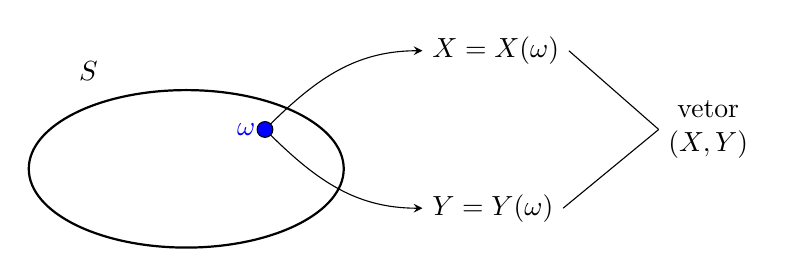
\begin{tikzpicture}
        \draw[thick] (-3, 0) ellipse[x radius=2, y radius=1];
        \node[anchor=south east] at (-4, 1) {$S$};

        \coordinate (P) at (-2, 0.5);
        \coordinate (X) at (0, 1.5);
        \coordinate (Y) at (0, -0.5);
        \coordinate (V) at (3, 0.5);
        
        \node[anchor=east, blue] at (P) {$\omega$};
        \node[anchor=west] (Xw) at (X) {$X = X(\omega)$};
        \node[anchor=west] (Yw) at (Y) {$Y = Y(\omega)$};
        \node[anchor=west, align=center] at (V) {vetor\\$(X, Y)$};
        
        \draw[->,>=stealth] (P) to [out=45,in=180] (X);
        \draw[->,>=stealth] (P) to [out=-45,in=180] (Y);

        \draw (Xw.east) to (V);
        \draw (Yw.east) to (V);

        \draw[fill=blue] (P) circle (0.1);
    \end{tikzpicture}
\end{center}

\begin{example}\label{exp:ch03-dois-dados}
    Dois dados são lançados. Temos
    \begin{align*}
        S &= \{
            (i, j) : 
            i \in \{1, \cdots, 6\},\ 
            j \in \{1, \cdots, 6\}
        \}
    \end{align*}

    Para $\omega = (i, j) \in S$, definimos:
    \begin{align*}
        X = X(\omega) &= i + j \\
        Y = Y(\omega) &= \min(i,  j)
    \end{align*}

    Desta maneira, $(X, Y)$ é um vetor aleatório
    cuja primeira componente representa a soma
    dois resultados mostrados pelos dois dados
    e a segunda componente representa o mínimo
    destes resultados.
\end{example}
